% Overleaf: compile with pdfLaTeX. Self-contained (no .bst needed).
\documentclass[11pt,a4paper]{article}
\usepackage[utf8]{inputenc}
\usepackage[T1]{fontenc}
\usepackage{lmodern}
\usepackage[margin=2.5cm]{geometry}
\usepackage{amsmath,amssymb}
\usepackage{graphicx}
\usepackage{booktabs}
\usepackage{array}
\usepackage{tabularx}
\usepackage{caption}
\usepackage{setspace}
\usepackage{microtype}
\usepackage[numbers,sort&compress]{natbib}
\usepackage[hidelinks]{hyperref}
\usepackage{lineno}
\linenumbers
\onehalfspacing
\captionsetup{font=small,labelfont=bf}
\renewcommand{\arraystretch}{1.15}
\graphicspath{{figures/}}
\newcolumntype{L}[1]{>{\raggedright\arraybackslash}p{#1}}
\newcommand{\Ce}{\textit{C.~elegans}}

\title{What an atlas-fitted connectome can and cannot do: evolutionary search over interneuron stimulation in a whole-body \Ce{} model}
\author{Taehee Lee\\[2pt]
\small Department of Integrative Medicine, Yonsei University, Seoul, Republic of Korea\\
\small Correspondence: \texttt{kairess87@gmail.com}}
\date{}

\begin{document}
\maketitle

\section*{Abstract}
The \Ce{} connectome is complete, but which behaviours its wiring can produce, and which it cannot, is unknown. We asked this question in a whole-body simulation whose only adaptive element is a learning agent outside the nervous system. The agent may inject current into a short whitelist of interneurons, never into motor neurons or muscles; the 302-neuron OpenWorm c302 network, with dynamics fitted once to a signal-propagation atlas, a literature-based motor layer and a viscoelastic body on agar do the rest. Every hypothesis was pre-registered with its judgement criterion. Stimulating five command and steering interneurons (AVB, AVA, SMDD, SMDV, RIV) was sufficient for chemotaxis to a source 2.5~mm away (91\% of trials; four of five training seeds), whereas stimulating eight sensory neurons was no better than chance, reproducing at the behavioural level the silence of the sensory-to-command step in the fitted network. Evolution rediscovered the pirouette rule, reversing and executing a deep bend when concentration fell, and ablations showed that reversal, deep bend and steering were all necessary. Shuffling the wiring while preserving weights, counts and signs cut performance to a fifth; in the atlas-fitted dynamics this loss was carried by the gap-junction layer. In corridors four body widths wide, corners were passed only by a deep bend pressed against the wall, so the dorsal or ventral direction of the bend fixed the direction of the turn. With ventral bends only, right turns were impossible and the worm always entered the ventral arm of a T-maze. Because temporal sensing cannot distinguish the arms at a junction, the learned strategy was to enter one arm and reverse when the odour faded; a left--right concentration difference was needed before the bend direction followed the source. The model yields three testable predictions for narrow-maze assays and separates what the wiring contributes to navigation from what sensing and the body must supply.

\section*{Author summary}
Knowing every connection in a nervous system does not tell us what the wiring does. We took the complete wiring diagram of the worm \Ce{}, kept every connection fixed, and let a learning algorithm discover what it could achieve by stimulating a handful of neurons, as an experimenter with optogenetic tools could. The algorithm was forbidden to touch the neurons that drive muscles. Through the wiring it learned to find an odour source, and it did so by rediscovering the strategy real worms use: reverse and turn sharply when the smell gets weaker. It failed when given only sensory neurons, which tells us that the sensory-to-command step is missing from the fitted wiring. Randomising the wiring destroyed the behaviour, and in our fitted model the electrical connections were the ones that mattered. In narrow mazes, the worm could only turn toward the side of its sharp bend, so a worm that bends to one side always turns that way and needs a costly reversal to reach food on the other side. These results separate what the wiring contributes from what the body and the senses contribute, and they make predictions that can be tested with worms in mazes.

\section*{Introduction}
The wiring diagram of \Ce{} has been complete for decades \cite{r4,r5}, but a wiring diagram is not a functional model, and the electrophysiological parameters that would turn one into the other are largely unknown \cite{r1,r6}. Two responses to this gap dominate. One fits network dynamics to measured signal propagation; the recent atlas of Randi et al.\ showed that anatomy alone predicts only part of the functional map \cite{r2}. The other fills the unknown parameters by optimisation against behaviour and obtains an ensemble of models consistent with anatomy \cite{r1}. Both ask what the wiring \emph{does}. Here we ask a complementary question: with the wiring fixed and the free parameters confined to a learning agent outside the nervous system, which behaviours can be produced through the connectome, and which cannot?

We built a whole-body simulator in which the OpenWorm c302 network \cite{r6} is coupled to the neuromechanical motor layer of Boyle, Berri and Cohen \cite{r7} and to a two-dimensional viscoelastic body crawling on agar, with walls. The network dynamics were fitted once to the signal-propagation atlas \cite{r2} and then frozen. A small policy, trained by evolution strategies \cite{r8}, observes the odour at the nose and may inject current into a whitelist of sensory, command and steering interneurons. It may never stimulate motor neurons or muscles. Behaviour therefore arises only from what the stimulated interneurons can do through the fixed wiring, the situation of an optogenetic experiment on a circuit whose downstream connectivity cannot be changed.

This framing turns the fitted connectome into an experimental subject. Because the agent adapts and the model does not, a failure to learn a behaviour is evidence about the fitted network rather than about a hand-tuned controller, and a success identifies which interneurons are sufficient. It also lets us compare the learned strategy with those of real animals. Chemotaxis in \Ce{} is produced by pirouettes, sharp reorientations whose probability rises when the concentration falls \cite{r9}, and by a weathervane mechanism that steers gradually toward higher concentration \cite{r10}. Sharp reorientations are executed by a stereotyped neural sequence in which SMD and RIV drive the omega bend and SMDD versus SMDV set its dorsal or ventral direction, which the animal chooses according to the odour gradient \cite{r11}. Real animals in narrow T-mazes show no innate side bias and find a food arm in 85\% of trials, a behaviour that requires mechanosensation \cite{r3}. These anchors let us judge whether an agent constrained by the connectome converges on the same solutions.

We pre-registered each hypothesis with its judgement criterion before training and kept every negative result. We report that five command and steering interneurons suffice for chemotaxis while sensory neurons do not; that evolution rediscovers the pirouette rule and that reversal, deep bend and steering are all required; that in narrow corridors the direction of the deep bend is the direction of the turn, which makes arm choice at a T-junction a problem of bend direction and lateral sensing rather than of the connectome; and that the real wiring outperforms shuffled wiring through its gap-junction layer.

\section*{Results}

\subsection*{The agent's only lever is current into whitelisted interneurons}
Everything downstream of the stimulated neurons is fixed (Fig~\ref{fig1}). Every 0.5~s a small neural-network policy maps the recent history of log odour concentration at the nose, and in maze tasks the wall contact of the head, to currents of 0--6~pA injected into the chosen neurons of the c302 network (302 neurons, 2,279 neuron-to-neuron chemical synapses, 1,084 gap junctions) with dynamics fitted to the signal-propagation atlas \cite{r2} (``Vfit'', Methods). The motor layer reads only five interneurons. Forward and backward locomotion are gated by AVB and AVA depolarisation \cite{r7}; the SMDD~$-$~SMDV difference steers the head; and a RIV depolarisation above threshold fires a travelling curvature pulse that produces an omega turn of about 170$^\circ$, which we call the deep bend \cite{r11}. Under the rule adopted for maze experiments, the pulse is dorsal when SMDD exceeds SMDV and ventral otherwise, as in the neural sequence of directed turning \cite{r11}; the earlier ventral-only rule serves as a control. The two rules are recorded as architecture decision records ADR-016 and ADR-017 (Methods). Policies were trained by evolution strategies with a near-source curriculum and evaluated on 128--256 fresh random starts. Hypothesis identifiers (H1, H5-3, \ldots) refer to Table~\ref{tab1}.

\subsection*{Five command and steering interneurons suffice for chemotaxis; sensory neurons do not}
Stimulating only AVB, AVA, SMDD, SMDV and RIV was sufficient for chemotaxis (Fig~\ref{fig2}A). The trained policy reached a source 2.5~mm away within 40~s in 91.4\% of 256 trials (Wilson 95\% CI 0.873--0.943; median 24~s), against 4.3\% for a random policy and 0\% for a still worm; at 1.5~mm it reached 99.6\%. Four of five independent training seeds cleared the pre-registered criterion of 0.8 (0.914, 0.973, 0.969 and 0.934; mean of five $0.82 \pm 0.29$ s.d.). The remaining seed converged to a strategy that reversed on decline but never used the deep bend, reached 0.301, and stayed there after 100 further generations (0.324); we return to this local optimum below. An oracle controller that knew the source direction and steered the same body directly reached the source in 89.5\% of trials, fewer than the learned policy, though faster (median 16.5~s versus 24~s). The oracle is a hand-tuned baseline, so we conclude only that the interneuron interface costs nothing in reach rate, not that it is optimal. Learning failed without three ingredients that we record as negative results: a living cost and a terminal distance penalty (otherwise standing still is a local optimum), relative rather than absolute concentration observations, and the curriculum (direct training at 2.5~mm reached 8\% after 45 generations).

Stimulating sensory neurons instead of interneurons did not produce chemotaxis. With ASE, AWC, AWA, ASK, ASH, PLM, ALM and AVM as the only channels, the best policy reached a source 1.5~mm away in 10.9\% of trials (CI 0.077--0.154), against 12.5\% for a random policy (CI 0.090--0.171), and its learning curve stayed at the reward of a still worm for 80 generations. The policy had tried to exploit a sub-millivolt asymmetry of the touch circuit, with the sign opposite to the biological one. This behavioural failure matches two properties of the fitted network established when it was built (Methods): static sensory stimulation does not differentiate the forward and backward command states, and 83\% of the inhibitory responses in the atlas connect neuron pairs that have no one- or two-step synaptic path. The gap between the two conditions at 1.5~mm, 0.996 versus 0.109, is the contribution of the single missing step, sensory-to-command selection.

\subsection*{Evolution rediscovers the pirouette rule, and reversal, deep bend and steering are all necessary}
The learned policy implemented the pirouette rule of Pierce-Shimomura et al.\ \cite{r9} (Fig~\ref{fig2}B--C). Sweeping the policy over the observed concentration change gave a clean switch. When concentration fell, AVA (reverse) was driven at 0.98 of maximum with a ventral head bias (SMDV 0.83); when it rose, AVB (forward), RIV (deep bend) and SMDD were driven at 0.89, 1.0 and 0.99. The rate of reversal onsets fell monotonically across quintiles of $\mathrm{d}C/\mathrm{d}t$, from 0.533 to 0.056 per second (ratio $\approx 9$, Spearman $\rho = -0.90$), the sign and monotonicity reported for real animals \cite{r9}. The model's baseline rate (0.23 per second) is 8--10 times the real one (0.023--0.030 per second \cite{r9}) because its reversal bouts are short (2~s) and frequent. The other successful seeds implemented the same switch with different weights. In all four navigating seeds the realised probability of the backward gate was highest in the falling quintile and lowest in the rising one (0.15~$\to$~0.09, 0.30~$\to$~0.04, 0.50~$\to$~0.02 and 0.31~$\to$~0.03), but the onset-rate statistic, which counts AVA crossings of half maximum, was monotone in only two of them ($\rho = -0.90$ and $-0.70$; $-0.30$ and $+0.70$ in the others). The seed with the positive value reversed by switching AVB off while holding AVA near half maximum, so that the backward gate won without an AVA crossing. The rule is therefore reproduced at the level of gating in every navigating seed, and the crossing-based onset rate is a readout that depends on how the policy implements it. The weathervane mechanism \cite{r10} did not appear: the sign of head steering agreed with the side of the source in 0.27 of steps (criterion $>0.7$), because steering was tied to $\mathrm{d}C/\mathrm{d}t$, not to the gradient direction, which a nose sampling only the temporal history cannot observe.

The rule alone was not sufficient. Restricting the channels to AVB, AVA and RIV, the pre-registered condition for the rule test, produced the rule in its purest form, reverse plus deep bend on decline and forward run on rise ($\rho = -1.00$), in two of three seeds, yet these policies could not navigate (reach 0.05--0.11 at 2.5~mm). Without steering the only reorientation is a fixed bend of about 170$^\circ$, so the worm retraces its path. The third seed of this rule test found an alternative, a bend held continuously during runs, that reached 0.328.

All three components were necessary (Fig~\ref{fig3}). Masking one channel of the trained policy at evaluation reduced the reach rate from 0.914 to 0.098 (AVA), 0.066 (RIV), 0.273 (SMDD and SMDV together), 0.434 (AVB) and 0.410 or 0.621 (SMDD or SMDV alone). Retraining without RIV reached 0.191 and retraining without steering 0.05, so the necessity is not an artefact of the particular policy. Our pre-registered prediction that the deep bend would be dispensable on open ground was therefore false: with temporal sensing only, chemotaxis by modulating the rate of reorientation (klinokinesis) requires a large reorientation. A further pre-registered hypothesis asked whether the sleep-active neuron RIS \cite{r17} would be recruited to stop at the source. It was not. When the task rewarded dwelling at the source, with or without a movement cost, the policy stopped by withdrawing command drive below the gate threshold and RIS stimulation stayed at zero; RIS can only matter when the forward drive is not under the agent's control.

\subsection*{In narrow corridors the direction of the deep bend is the direction of the turn}
Corners were passed by one mechanism only: a deep bend pressed against the wall (Fig~\ref{fig4}). We added a wall potential to the body model and lattice mazes with corridors 0.3~mm wide, about four body widths. In corridors of this width the omega bend, whose free diameter is 0.34~mm, is blocked (reorientation $+2^\circ$ instead of $+170^\circ$) and forward speed halves (0.07--0.10 versus 0.15--0.18~mm/s). Yet the odour policy trained on open ground, placed in an L-shaped corridor without further training, passed the corner in 100\% of 128 episodes. Frame-by-frame traces showed the sequence stall $\to$ reversal $\to$ forward run with a deep-bend pulse pressed against the wall, after which the body slides around the corner. In a 64-episode subset analysed step by step, a reversal command and a bend pulse both occurred within the 3~s before every corner passage (64 of 64), for the open-ground policy and for a maze-trained policy alike. Head steering alone could not turn the corner: constant SMDD or SMDV bias with forward drive passed 0 of 32 corners, and masking RIV reduced T-maze completion to 0.

The wall converts a blocked omega turn into a slide along the open side, so the dorsal or ventral direction of the bend is the direction of the turn (Fig~\ref{fig5}). Under the ventral-only rule, policies passed left-turn corridors in 32 of 32 trials and right-turn corridors in 0 of 32, at corridor widths of 0.25, 0.30 and 0.35~mm, and entered the left (ventral) arm of a T-maze first in 128 of 128 trials regardless of where the food was. A $3\times3$ grid maze that requires two right turns was unsolvable in principle. Under the SMD-direction rule, which permits dorsal bends through whitelisted stimulation, retraining on the right-turn corridor succeeded (reach 1.00) but produced a one-handed policy that failed the left-turn corridor (0.00), and policies not trained on right turns kept turning left. The rule preserved open-ground chemotaxis (0.871, CI 0.824--0.907). The retrained open-ground policy used dorsal bends 0.77 of the time and ventral bends 0.11, the opposite of real animals, in which 24\% of sharp turns are dorsal \cite{r12}. The model has no dorsal--ventral cost asymmetry, so its preferred direction is set by initialisation; the ventral preference of real worms lies outside what this model can explain.

\subsection*{At a T-junction temporal sensing cannot choose the arm, so the policy enters one arm and reverses when wrong}
Policies trained in the T-maze reached the food in 100\% of trials and finished in the food arm in 100\%, but they never chose the arm at the junction. First entry was into the left arm in 128 of 128 trials under both bend rules, and food on the right cost 7--38~s more than food on the left across policies (22~s versus 40~s for the first maze-trained policy). The correction was not a discrete choice but repeated 2~s reversal bouts that carried the worm tail-first back through the junction and into the other arm. Wall-contact observations were unnecessary. Zeroing them at evaluation left reach and arm choice at 1.00 and shortened the median time from 40~s to 30~s; a policy trained with odour only performed identically (1.00), whereas the open-ground policy without maze training reached 0.49 and a policy trained with contact only converged to stillness (0.00). In this model the ``multisensory'' requirement of real maze navigation \cite{r3} is met by odour plus wall physics, not by wall sensing.

The reason is informational. At the junction both arms present the same concentration to a nose that senses only the temporal history, so the correct arm can be found only by entering one. Adding proprioception (head curvature) made navigation faster (T-maze median 26.5~s) but did not change first entry (128 of 128 left); the policy used curvature to time the deep bend to the head-swing phase. The pre-registered prediction that dorsal bends would let the policy choose the arm (H5-6) was rejected: dorsal bends give the repertoire, not the decision.

The stall reflex that takes corners also aborts a correctly aimed right entry. Recording body frames at the junction showed that a dorsal pulse carried the head into the right arm to $x \approx 0.45$~mm, where it stalled against the wall. The stall registered as a weak fall in concentration ($\Delta \log C$ of $-0.13$ to $-0.15$ per step), which triggered the open-ground reflex, reverse with a ventral head bias, and returned the worm to the left arm. Gating that reflex off during frontal wall contact abolished all cornering (reach 0.00), and masking SMDV or AVA at the junction reduced completion to 0.00 and 0.50. The same reflex is thus the means of turning corners and the cause of the aborted entry.

\subsection*{Lateral concentration information selects the bend direction}
When the observation included the log-concentration difference between two points 0.1~mm to the left and right of the nose, an idealisation of the head-swing sampling of real animals, the policy used it (Fig~\ref{fig6}A). On open ground it reached the source in 98.8\% of trials with a median of 16.5~s, the speed of the oracle. It used both bend directions (2,180 dorsal and 3,251 ventral pulses in 128 episodes), and the realised direction of the deep bend matched the side of the source in 0.73 of pulses, against 0.62 for the same rule without lateral information (chance 0.5). Because pulses within an episode are not independent, we recomputed the statistic per episode: $0.73 \pm 0.08$ (all 128 episodes above 0.5) versus $0.61 \pm 0.18$ (88 above, 35 below, 5 at 0.5), Mann--Whitney $p = 2.6 \times 10^{-8}$, Cohen's $d = 0.85$. This reproduces, in the model, the sensory-guided choice of dorsal versus ventral turns reported for real animals \cite{r11}. In the T-maze, however, the lateral-information policy still entered the left arm first in 128 of 128 trials. At the junction it fired dorsal pulses toward a right-hand goal in 0.80 of cases, but each entry was aborted by the stall reflex described above; the maze-trained version abandoned dorsal pulses and instead reduced the cost of a right-hand goal to 7~s.

\subsection*{The real wiring outperforms shuffled wiring, through its gap junctions}
The wiring contributed even though the command neurons were stimulated directly (Fig~\ref{fig6}B). We shuffled the postsynaptic targets of all neuron-to-neuron chemical synapse entries (3,364 after sign splitting, Methods) and one end of all 1,084 gap junctions, preserving every weight, count and sign, and retrained under the same curriculum and rules. Three shuffled networks reached 0.141, 0.145 and 0.320 (mean 0.202) against 0.871 for the real wiring, and the real-wiring policy transferred to the shuffled networks reached 0.023--0.055. The deficit tracked the deep bend: in 128 evaluation episodes the real network fired 6,960 pulses, the three shuffled networks 0--38, 670 and 3,599, in the same order as their reach rates. Direct stimulation raises the potential of the stimulated neuron regardless of wiring, so the wiring's contribution lies in how the stimulus spreads to the readout neurons SMD and RIV.

In the fitted dynamics that contribution was carried by the gap-junction layer. Shuffling only the chemical synapses left performance intact (retrained 0.859, transferred policy 0.914, 6,493 pulses), whereas shuffling only the gap junctions collapsed it (0.078 and 0.125, 116 pulses); the confidence intervals of the two layer-specific controls do not overlap (Table~\ref{tab2}). The fit to the atlas had scaled chemical conductances down by more than an order of magnitude while leaving gap junctions near unity (Methods), so the neuron-to-neuron chemical layer is nearly silent in this model by construction. The defensible statement is therefore about the atlas-fitted dynamics: in them, the stimulus reaches SMD and RIV through the gap-junction network.

\subsection*{The reported numbers are robust to integration precision}
All headline numbers held at the fine integration step required by our reporting rule. Headline values are those measured at the training step (0.25~ms, single precision) on 256 starts. On a common set of 128 starts, integrating at 0.05~ms in double precision gave reach rates of 0.914 (versus 0.938 at the coarse step) for the open-ground policy, 0.875 (versus 0.844) for the SMD-direction policy, and 1.00 with 128 of 128 left first entries under both settings for the maze-trained SMD-direction policy; only its maze transit time changed (median 26.5~$\to$~33.5~s). Wilson 95\% confidence intervals for the key comparisons are given in Table~\ref{tab2}.

\section*{Discussion}
The central result is a partition. Inside the fitted connectome lie the sufficiency of five command and steering interneurons for chemotaxis, the necessity of reversal, deep bend and steering together, and a contribution of the wiring that is carried by gap junctions. Outside it lie the sensory-to-command step, which the fitted network does not perform, and the two ingredients that decide arm choice in a narrow maze, the dorsal--ventral direction of the deep bend and a lateral sample of the gradient. The model does not say that the connectome is unimportant for these. It says that in an atlas-fitted network with a literature motor layer they must be supplied from elsewhere, and it names what they are.

The learned strategy converged on the pirouette rule of real animals \cite{r9} without being told it, under the narrowest channel set (AVB, AVA, RIV) as well as the full one. Convergence was not sufficiency. A run-and-tumble policy with a fixed reorientation of about 170$^\circ$ cannot navigate, and every successful policy combined the rule with SMD steering that modulates the bend angle; real pirouettes likewise combine reversals with omega turns of variable angle \cite{r9,r13}. The convergence suggests that the rule is a property of the task and of the motor repertoire rather than of a particular circuit. The necessity of a deep bend follows from temporal sensing, as the lateral-information experiment showed: with a left--right sample the worm went straight to the source at the oracle's speed, using the weathervane mechanism \cite{r10} in the form of bend direction rather than of continuous steering. Our failure to learn a weathervane from proprioception plus temporal sensing at a 0.5~s decision interval is consistent with the head-swing sampling of real animals being faster than our observations.

The wiring-shuffle controls answer a natural objection: if the agent stimulates command neurons directly, perhaps the wiring is irrelevant. It is not. Random wiring with identical weights, counts and signs performed at a fifth of the real wiring after retraining, and the loss was exactly the loss of deep-bend pulses, that is, of the spread of stimulation to RIV and SMD. The layer dissociation, intact with shuffled chemical synapses and collapsed with shuffled gap junctions, has a clear caveat: the atlas fit had already reduced chemical conductances thirty-fold. We therefore claim a property of the fitted dynamics, not of the animal. It is, however, the same property that the atlas reported directly, that gap junctions and extrasynaptic signalling explain much of what anatomy alone does not \cite{r2}, which suggests that the fit and the shuffle test probe the same structure. Whether the chemical layer becomes necessary under a different fit is a question the pipeline can answer; our own attempt with separate inhibitory operating points did not improve validation and was recorded as negative.

The maze results make three predictions for real animals. First, in T-mazes with corridors a few body widths wide, the arm entered should be predicted by the dorsal or ventral direction of the omega bend executed at the junction, which can be read from high-speed video. Second, conditions that suppress dorsal turns, whose spontaneous fraction is about 24\% and falls to 16\% during boundary escape \cite{r12}, should bias animals toward the ventral arm and delay reaching a goal in the other arm; the wild-type absence of side bias (decision index 0.03 \cite{r3}) then requires that dorsal bends be used at the junction at a compensating rate. Third, stalling against a wall should trigger a pirouette, because in the model the same reflex that takes corners aborts a wrongly aimed entry. The model also reinterprets the mechanosensory requirement of maze navigation \cite{r3}. Wall-contact observations were unnecessary for our agent, so the failure of \textit{mec-4} mutants may instead reflect the use of wall contact for propulsion \cite{r14} or for memory formation rather than for arm choice, a distinction that can be tested by separating the two.

The model has limits that bound these claims. The motor layer, steering and deep-bend rules are literature-based assumptions outside the connectome; each is anchored to a published mechanism \cite{r7,r11}, but their parameters were chosen, not fitted. The body has no wall-pushing propulsion \cite{r14}, so it crawls slowly in corridors, and it has no dorsal--ventral cost asymmetry, so it cannot explain the ventral preference of real turns. Sensory neurons are stimulated as currents, not through odour transduction, so the negative sensory result is a statement about the fitted network, not about real sensory neurons. Odour passes through walls. One learning algorithm and one small policy were used, and the $3\times3$ grid maze had no robust solution, only an open-loop sequence that failed under start jitter. One of five training seeds converged on a reversal-only local optimum; the sufficiency claim concerns the existence of solutions through the wiring, which four seeds and every ablation confirm, not the reliability of evolution strategies.

The approach treats a connectome as something to be interrogated by an adaptive experimenter rather than as a parameter set to be tuned. Its answers are of two kinds. Positive ones, such as the sufficiency of a command-interneuron interface, identify minimal stimulation targets for behaviour. Negative ones, such as the silence of the sensory step or the impossibility of a right turn with ventral bends, identify where the model, or the animal, must contain something the wiring diagram does not show.

\section*{Methods}

\subsection*{Network model}
We used the OpenWorm c302 framework \cite{r6} at parameter level C2, which represents each of the 302 neurons and 95 body-wall muscle cells as a single compartment with leak, slow and fast potassium and calcium conductances, graded chemical synapses and ohmic gap junctions. We re-implemented its equations in JAX so that hundreds of worms can be integrated in parallel on a GPU. The reference network was generated by c302 as NeuroML from the published connectome \cite{r4,r5} and never edited: 2,279 neuron-to-neuron chemical synapses (2,079 excitatory and 200 inhibitory in the c302 defaults), 552 neuron-to-muscle synapses and 1,084 gap-junction entries, with synaptic weight equal to the number of anatomical contacts. Voltage is integrated by backward Euler and gating, synaptic and calcium variables by exact exponential updates; against NEURON the re-implementation agrees to 0.001~mV RMS at a step of 0.05~ms. Exploration and training used a step of 0.25~ms in single precision; the headline numbers were re-checked at 0.05~ms in double precision (Results).

\subsection*{Fitted dynamics (``Vfit'')}
Two modifications, recorded as decisions ADR-010 and ADR-011, define the working variant. First, the sign of each neuron-to-neuron chemical synapse was assigned from receptor and transmitter expression in the CeNGEN atlas \cite{r15} with the method of Fenyves et al.\ \cite{r16}; synapses with conflicting predictions (1,085 of 2,279) were split into an excitatory and an inhibitory half, giving 3,364 synapse entries. Second, six global parameters were fitted to the signal-propagation atlas of Randi et al.\ \cite{r2}: the log conductance scales of excitatory, inhibitory and gap-junction connections and of the neuronal leak, and the half-activation voltage and slope of the graded synapse. The atlas protocol was simulated as a 2~pA current for 500~ms in each of 172 stimulus neurons, with the response defined as the mean depolarisation over 2~s relative to an unstimulated control. The loss combined the negative Pearson correlation, a soft rank loss on the area under the receiver operating characteristic curve (AUROC) between significant and non-significant responder pairs, and a penalty on network-wide up-states; it was minimised by Adam (learning rate 0.1, 50 steps) on 32 stimulus neurons and validated on the remaining 140. The fitted values $\theta = [-3.44, -6.25, 0.13, 0.69, 1.48, 0.77]$ scale excitatory conductances by 0.032, inhibitory conductances by 0.002 and gap junctions by 1.14, double the leak, and shift the synaptic threshold to $+1.5$~mV with a slope of 10.8~mV. On the validation neurons the fitted model reached an AUROC of 0.646 (95\% CI 0.617--0.671) and a Spearman correlation of 0.131 (0.103--0.153), against 0.546 and 0.075 for anatomy alone; the split-half reliability of the atlas bounds the attainable correlation at 0.140. Lesioning the model showed that this predictive power comes from gap-junction diffusion (gap junctions alone 0.613, chemical synapses alone 0.552). Of the 150 significant inhibitory responses in the atlas, 124 (83\%) connect neuron pairs with no one- or two-step chemical or electrical path in the connectome and cannot be produced by any synaptic parameter setting. Under these dynamics, static stimulation of AVB or AVA differentiates B-type from A-type motor neurons, but stimulation of touch neurons does not differentiate the command state. Class-wise fits and separate inhibitory operating points overfit (validation correlation fell to $\approx 0$) and were rejected.

\subsection*{Body}
The body is a two-dimensional overdamped viscoelastic rod of 24 segments and 1.0~mm length lying on its side, so that dorsoventral bending is in-plane. Stretch stiffness is $5\times10^{4}$ and bending stiffness 5 in units normalised to the tangential drag coefficient, with a normal-to-tangential drag ratio of 40 for crawling on agar; the rod is integrated at 10~$\mu$s. With an imposed travelling wave the rod crawls at 0.24~mm/s. Muscle activation is mapped from the 24 rows of c302 muscle cells. Walls are line segments with a repulsive potential $\tfrac12 k_w (r_w - d)^2$ acting on any node closer than $r_w = 60$~$\mu$m ($k_w = 5\times10^{3}$); penetration was zero and results were stable for $k_w$ between $2\times10^{3}$ and $2\times10^{4}$. Wall contact of the four head nodes within 0.12~mm is reported to the policy as three numbers (left, right, front) between 0 and 1.

\subsection*{Motor layer and readouts}
The c302 motor circuit has no intrinsic oscillator: no cell oscillates in isolation and no relaxation-oscillator regime exists in its channel-density space. The motor neurons and muscles were therefore replaced by the neuromechanical model of Boyle, Berri and Cohen \cite{r7} (ADR-012): twelve bistable units per side with on and off thresholds of 0.75 and 0.25, stretch-receptor gain 2.0 over 25\% (forward) or 50\% (backward) of the body, a muscle time constant of 100~ms and a maximal curvature of 6~mm$^{-1}$, updated every 5~ms. Tuned in this way the body crawls at 0.18~mm/s at 0.50~Hz with head-to-tail propagation. Everything upstream of the command interneurons remains the fitted connectome. Four readouts couple the network to the motor layer, each anchored to a published mechanism. (i)~Gates (ADR-012): the forward or backward gate opens when the mean depolarisation of AVB or AVA relative to a 2~s unstimulated baseline exceeds 3~mV, the larger of the two winning. A quiescence gate for the sleep-active neuron RIS \cite{r17} stops the motor layer when RIS is depolarised by more than 3~mV and by more than 1.5 times any command or steering neuron. (ii)~Head steering (ADR-013): the resting curvature of the anterior twelve rows, and the reference curvature of their stretch receptors, is offset by 0.03~mm$^{-1}$ per mV of SMDD~$-$~SMDV depolarisation, giving turns of about $\pm 50^\circ$ in 12~s. (iii)~Deep bend (ADR-016): when the RIV depolarisation crosses 30~mV, a Gaussian curvature offset of width 4 rows and amplitude 0.36~mm$^{-1}$ per mV above threshold travels from head to tail over 2.5~s; the pulse fires on the rising edge and re-arms only after RIV falls below threshold. The threshold separates direct RIV stimulation ($\approx 55$~mV) from gap-junction leak of SMD stimulation ($\approx 20$~mV). (iv)~Direction (ADR-017): the pulse is dorsal when SMDD~$-$~SMDV exceeds 10~mV and ventral otherwise \cite{r11}. Network, motor layer and body exchange state every 50~ms.

\subsection*{Environment, observations and reward}
The odour is a two-dimensional Gaussian of peak 1 and width 2.0~mm centred on the source, evaluated at the nose; it passes through walls. On open ground the worm starts at the origin with a uniformly random heading and the source is placed at 1.5 or 2.5~mm in a uniformly random direction; in mazes the start pose and the goal are drawn from the stage's lists. An episode lasts 40~s (120~s in corridors and the T-maze, 150~s in the grid) and ends when the nose comes within 0.5~mm of the source. Every 0.5~s the policy observes the log concentration level and its changes over the preceding 0.5, 1.0, 1.5 and 2.0~s, scaled by 10. Where stated it also receives the three wall-contact values, the mean curvature of the six head joints, or ten times the log-concentration difference between points 0.1~mm to the left and right of the nose. The reward per step is $100\,\Delta C - 0.05$, plus 10 on reaching the source, minus 2~mm$^{-1}$ times the final distance if the source is not reached. In the dwelling task the episode continues after arrival with $+0.5$ per step inside the radius and an optional cost of 5 per mm of head movement. Mazes are lattices of open cells of side equal to the corridor width (0.3~mm; 0.25 and 0.35~mm in the width test): an L-shaped corridor with two 2.4~mm legs and one left or right corner, a T-maze with a 3.0~mm stem and 2.1~mm arms with the source at the end of one arm chosen at random, and a $3\times3$ grid of 1.2~mm pitch. The width was chosen because the omega turn completes at 0.4~mm but is blocked at 0.3~mm.

\subsection*{Policy, whitelist and training}
The policy is a multilayer perceptron with one hidden layer of 16 tanh units and a sigmoid output per channel; the output scales a constant current between 0 and 6~pA injected into every neuron of the channel (both members of a bilateral pair) for the whole 0.5~s step. The whitelist (ADR-002) contains 19 channels and 35 neurons: sensory (PLM, ALM, AVM, ASH, ASE, AWC, AWA, ASK), command (AVB, AVA, PVC, AVD), steering (SMDD, SMDV, RMDD, RMDV, RIV) and state (RIS, ALA). Motor neurons and muscles are never stimulated. The command and steering set used throughout is AVB, AVA, SMDD, SMDV, RIV; the sensory set is ASE, AWC, AWA, ASK, ASH, PLM, ALM, AVM; the rule test used AVB, AVA, RIV; the dwelling task added RIS. Policies were trained with OpenAI evolution strategies \cite{r8}: antithetic Gaussian perturbations ($\sigma = 0.2$) of the mean parameter vector, fitness averaged over a fixed set of episodes shared by all candidates, centred rank normalisation, and an update $\theta \leftarrow \theta + (0.1/\sigma)\,\overline{\epsilon F}$. Stage 1 used 32 candidates $\times$ 8 episodes for 40 generations at 1.5~mm; stage 2 used $64 \times 4$ for 100 generations at 2.5~mm from the stage-1 policy (60 generations for the SMD-direction chain and the wiring controls). Maze policies started from the open-ground policy with zero weights on the new inputs and used $32 \times 2$ for 40 generations. The training seed was 0 for the main results and 1--4 for replication; evaluation always used 128 or 256 fresh episodes with seeds disjoint from training. Ablations mask a channel's output at evaluation; sufficiency tests retrain without the channel.

\subsection*{Controls and statistics}
The wiring shuffles permute the postsynaptic neuron of every neuron-to-neuron chemical synapse entry (3,364) and one end of every gap junction (1,084) with a fixed seed, preserving each connection's weight, sign and kinetics, every presynaptic identity and out-degree, and all muscle connections; the layer-specific controls permute one class only. The oracle controller drives the motor layer directly with forward drive and a head bias proportional to the bearing to the source (gain 2, the best of the tested settings). A reversal onset is a step at which the AVA output crosses 0.5 upward; onset rates were computed within quintiles of the observed $\mathrm{d}C/\mathrm{d}t$ over 128 episodes. Realised bend direction is the sign of the deep-bend pulse at the step it fires, compared with the side of the source. Reach rates are given with Wilson 95\% confidence intervals; the per-episode bend-direction statistic uses a one-sided binomial sign test against 0.5 and a one-sided Mann--Whitney $U$ test between policies. All hypotheses, criteria and verdicts were written down before the corresponding training run and are listed in Table~\ref{tab1} and in the repository.

\subsection*{Code and data availability}
Simulator, training and analysis code, decision records, logs and figures are available at \url{https://github.com/kairess/worm-whisperer}; recorded simulations with neuron read-outs can be viewed at \url{https://kairess.github.io/worm-whisperer}.

\section*{Declaration of generative AI}
A generative AI coding assistant (Claude, Anthropic) was used to write and run the simulation and analysis code and to refine the English of the manuscript. All experiments, results and text were reviewed and verified by the author, who takes full responsibility for the content.

\section*{Funding}
This work received no specific funding.

\section*{Competing interests}
The author declares no competing interests.

% ---------------------------------------------------------------- Tables
\begin{table}[p]
\centering
\caption{\textbf{Pre-registered hypotheses and verdicts.} $n = 256$ episodes unless stated.}
\label{tab1}
\small
\setlength{\tabcolsep}{4pt}
\begin{tabular}{L{0.9cm} L{3.5cm} L{3.0cm} L{2.0cm} L{4.3cm}}
\toprule
ID & Hypothesis & Criterion & Verdict & Key numbers \\
\midrule
H1 & Command/steering channels suffice for chemotaxis & reach $\geq 0.8$ at 2.5 mm, random $\leq 0.2$ & \checkmark{} (4 of 5 seeds) & 0.914 / 0.973 / 0.301 / 0.969 / 0.934; random 0.043 \\
H1a & Sensory channels alone do not & not different from random & \checkmark & 0.109 vs 0.125 (1.5 mm) \\
H2-1 & Policy rediscovers the pirouette rule (AVB, AVA, RIV only) & $\rho(\mathrm{d}C/\mathrm{d}t,\ \text{reverse}) < -0.8$ & \checkmark{} rule / $\times$ sufficiency & $\rho = -1.00$; reach 0.05--0.11 \\
H2-2 & Weathervane steering with temporal sensing & steering sign = source side $> 0.7$ & $\times$ & 0.27 \\
H3 & Command layer is a low-cost interface & $\geq 70\%$ of oracle & \checkmark{} reach / $\triangle$ time & 0.914 vs 0.895; 24 vs 16.5 s \\
H4-1 & Deep bend dispensable on open ground & RIV ablation drop $< 0.1$ & $\times$ & $0.914 \to 0.066$; retrained without RIV 0.191 \\
H4-2 & RIS used to stop & RIS drive $> 0.1$ & $\times$ & 0.0 \\
H5-2 & Reversal, not bend, at corridor ends & AVA on frontal contact $\geq 0.6$ & $\times$ & corners taken by reversal \emph{and} bend (64/64) \\
H5-3 & Multisensory order in T-maze & odour+touch $>$ odour $>$ touch & \checkmark{} (touch observation unnecessary) & trained odour+touch 1.00 $>$ untrained odour-only 0.49 $>$ touch-only 0.00; trained odour-only 1.00 ($n = 128$) \\
H5-6 & Dorsal bends give arm choice & first entry = goal $> 0.7$ & $\times$ & 128/128 left \\
H5-8 & Lateral information is used & bend direction = source side $> 0.6$ & \checkmark{} (open ground) & 0.73 vs 0.62 \\
E5/E7 & Real wiring matters & shuffled $<$ real $- 0.5$ & \checkmark{} (gap junctions) & 0.202 vs 0.871; chemical-only 0.859, gap-junction-only 0.078 \\
\bottomrule
\end{tabular}
\end{table}

\begin{table}[p]
\centering
\caption{\textbf{Reach rates with Wilson 95\% confidence intervals} ($n = 256$, 2.5 mm unless stated). Rows with equal counts share an interval.}
\label{tab2}
\small
\begin{tabular}{L{6.4cm} L{3.4cm} L{4.8cm}}
\toprule
Condition & Reach & 95\% CI \\
\midrule
Full circuit (seed 0) & 0.914 & 0.873--0.943 \\
Full circuit (seeds 1--4) & 0.973 / 0.301 / 0.969 / 0.934 & 0.945--0.987 / 0.248--0.360 / 0.940--0.984 / 0.896--0.958 \\
Sensory channels only, 1.5 mm & 0.109 & 0.077--0.154 \\
Random policy, 1.5 mm / 2.5 mm & 0.125 / 0.043 & 0.090--0.171 / 0.024--0.075 \\
Real wiring, SMD-direction rule & 0.871 & 0.824--0.907 \\
All connections shuffled, retrained (3 seeds) & 0.141 / 0.145 / 0.320 & mean 0.202 \\
All shuffled, transferred policy (3 seeds) & 0.023 / 0.055 / 0.047 & \\
Chemical synapses shuffled, retrained / transferred & 0.859 / 0.914 & 0.812--0.896 / 0.873--0.943 \\
Gap junctions shuffled, retrained / transferred & 0.078 / 0.125 & 0.051--0.117 / 0.090--0.171 \\
Lateral-information policy & 0.988 & 0.966--0.996 \\
AVB/AVA/RIV only, bend-always seed & 0.328 & 0.274--0.388 \\
Retrained without RIV & 0.191 & 0.148--0.244 \\
\bottomrule
\end{tabular}
\end{table}

% ---------------------------------------------------------------- Figures
\begin{figure}[p]
\centering

\includegraphics[width=\textwidth]{fig1_pipeline.png}
\caption{\textbf{The pipeline and the whitelist principle.} Observation $\to$ policy $\to$ stimulation of whitelisted interneurons $\to$ fixed c302 connectome with fitted dynamics $\to$ literature motor layer $\to$ viscoelastic body in an odour field with walls.}
\label{fig1}
\end{figure}

\begin{figure}[p]
\centering
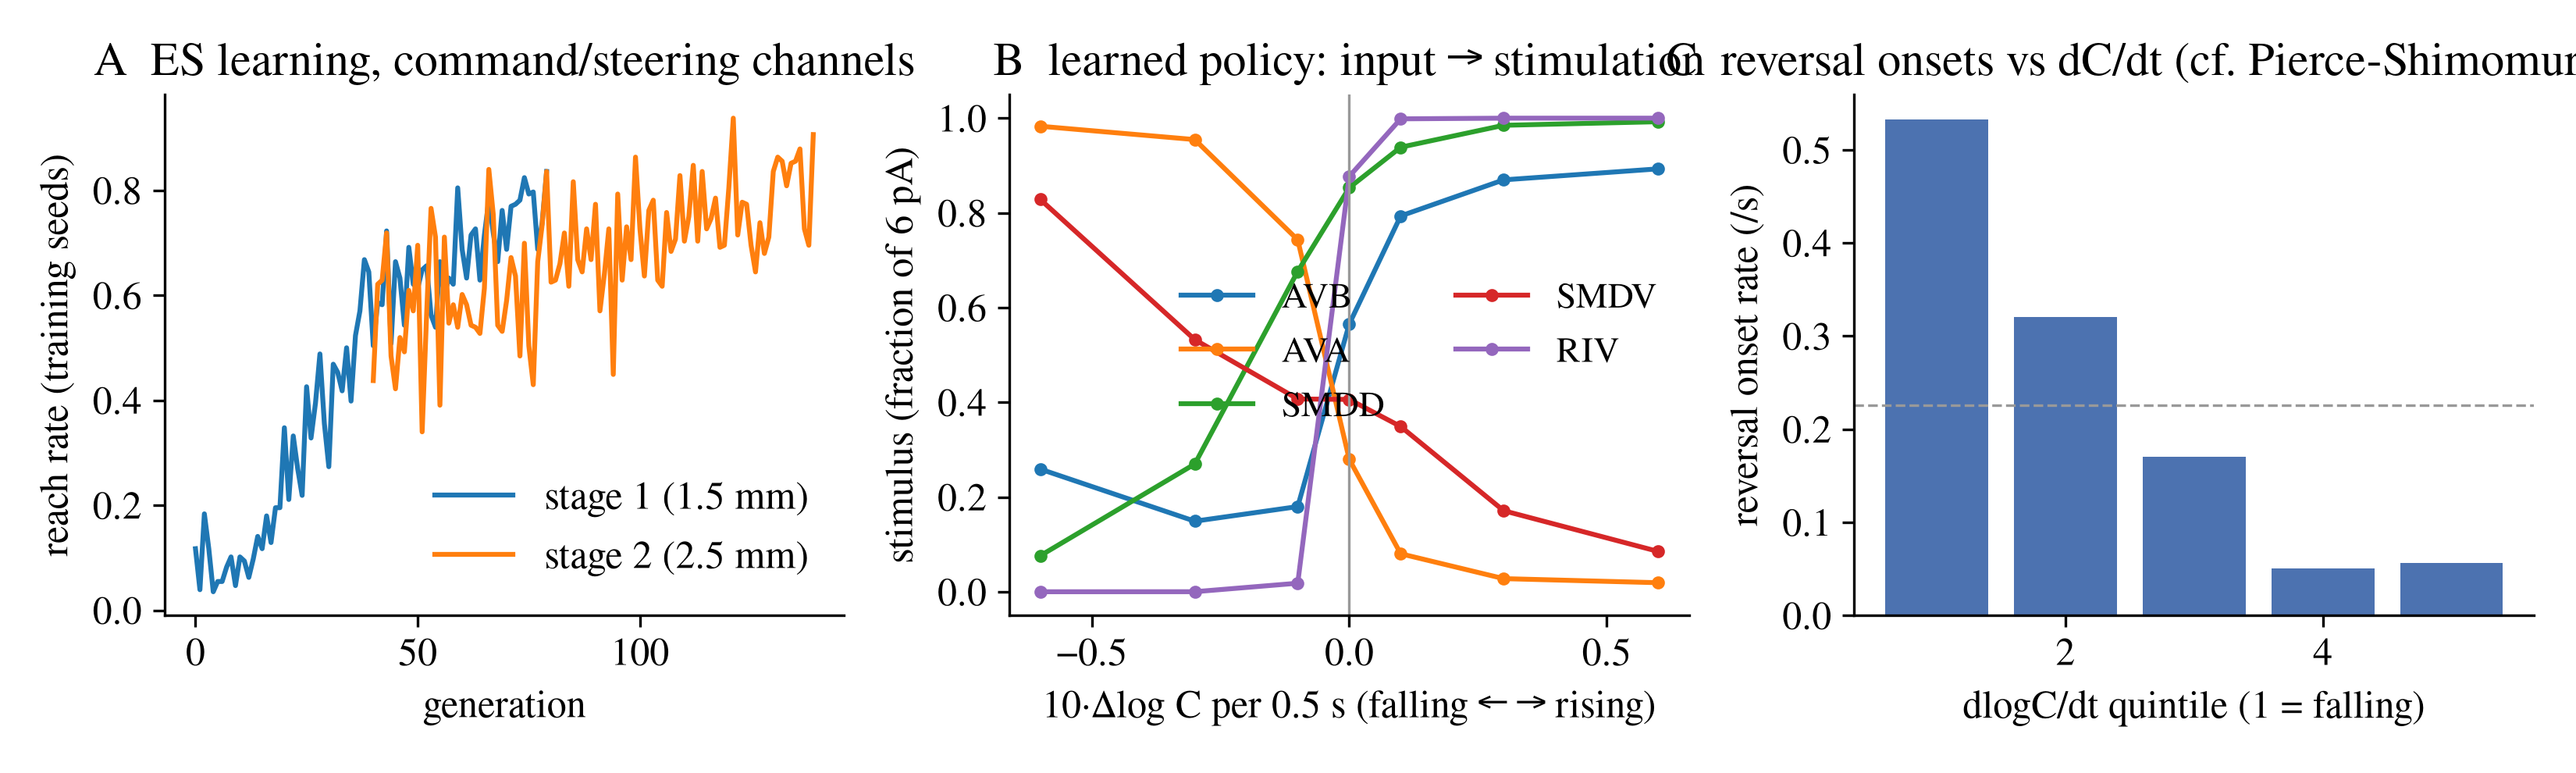
\includegraphics[width=\textwidth]{fig2_learning_and_rule.png}
\caption{\textbf{Chemotaxis through command and steering interneurons.} (A) Reach rate of the training seeds over generations under the curriculum (stage 1 at 1.5 mm, stage 2 at 2.5 mm). (B) Policy sweep: stimulation of each channel as a function of the observed concentration change. (C) Reversal-onset rate by $\mathrm{d}C/\mathrm{d}t$ quintile (1 = falling); the dashed line is the overall rate. Compare Pierce-Shimomura et al.\ \cite{r9}.}
\label{fig2}
\end{figure}

\begin{figure}[p]
\centering
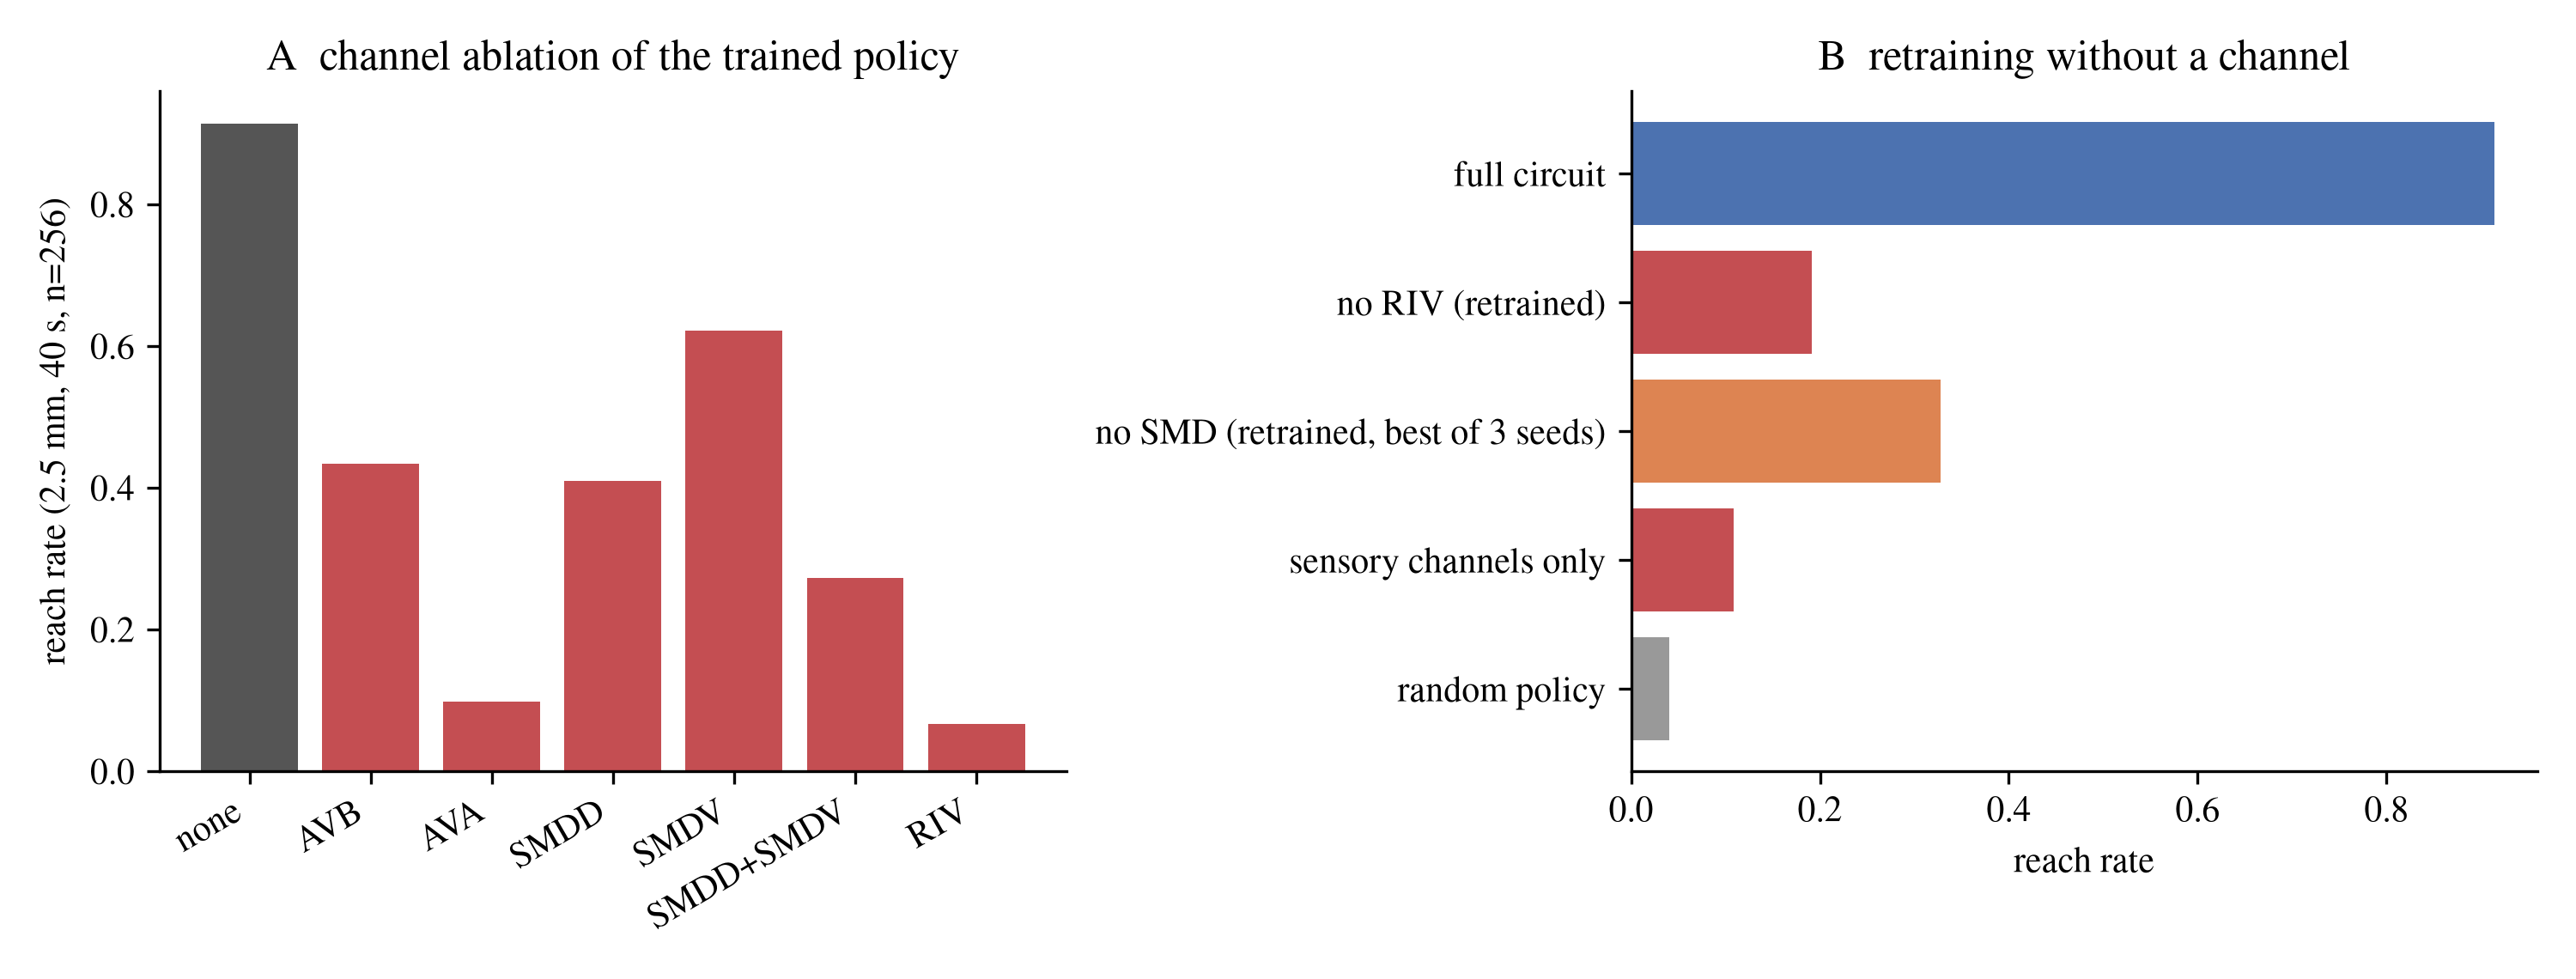
\includegraphics[width=0.8\textwidth]{fig3_minimal_circuit.png}
\caption{\textbf{The minimal circuit.} (A) Reach rate at 2.5 mm ($n = 256$) after masking each channel of the trained policy. (B) Reach rate after retraining without RIV or without SMD steering (best of three seeds), with the sensory-only and random policies for comparison.}
\label{fig3}
\end{figure}

\begin{figure}[p]
\centering

\includegraphics[width=\textwidth]{fig4_mazes.png}
\caption{\textbf{Mazes.} Recorded trajectories of the open-ground policy in the L-corridor, of the maze-trained policy in the T-maze with food on the left and on the right, and of the right-turn-trained policy under the SMD-direction rule in the right-turn corridor. Dorsal and ventral deep-bend pulses are marked along the head path; the dashed circle is the goal radius.}
\label{fig4}
\end{figure}

\begin{figure}[p]
\centering
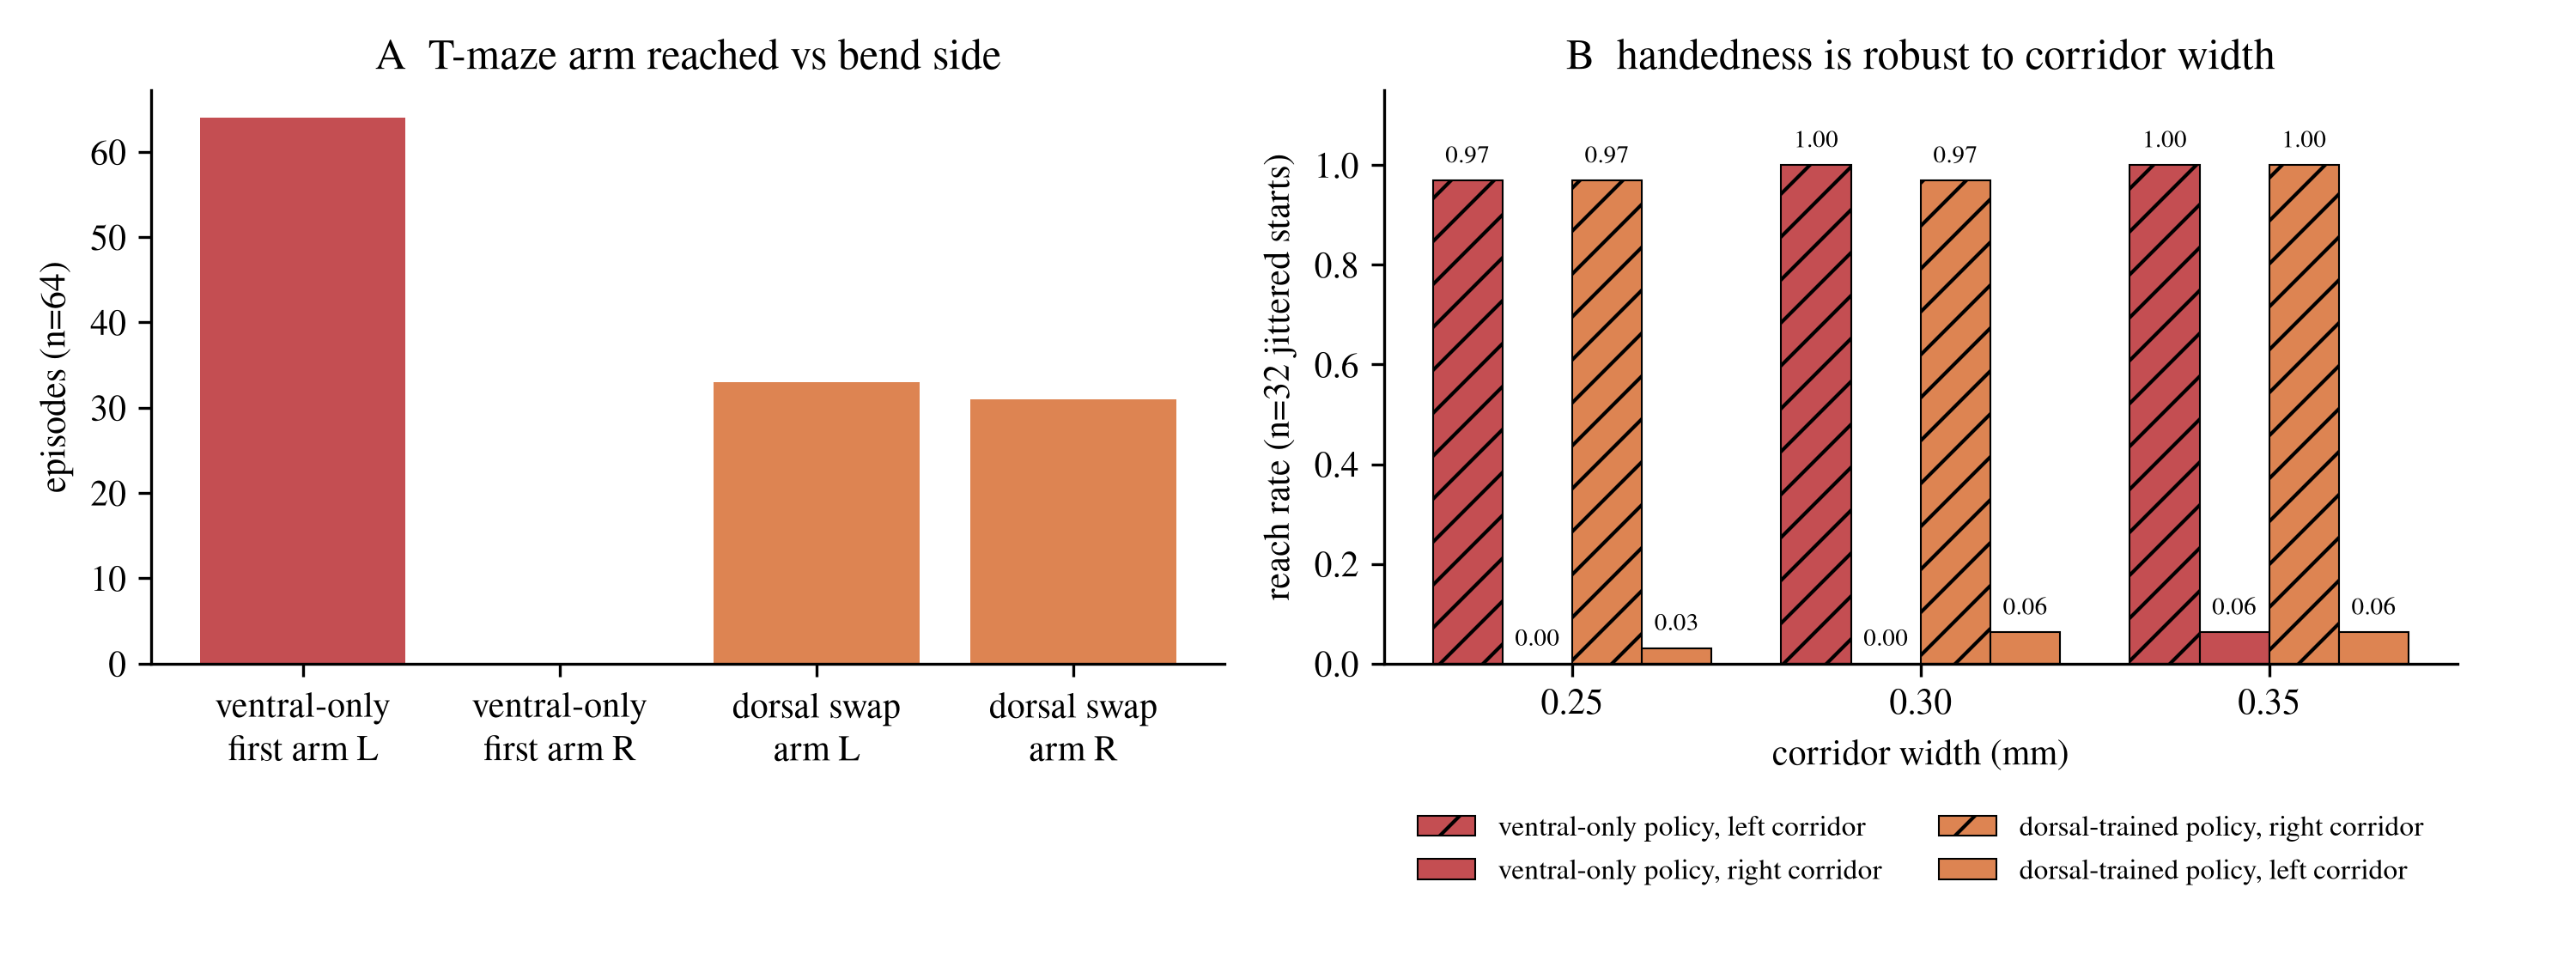
\includegraphics[width=\textwidth]{fig5_bend_direction.png}
\caption{\textbf{Bend direction is turn direction.} (A) First arm reached in the T-maze by the open-ground policy with ventral-only bends and with the bend direction swapped to dorsal ($n = 64$ each). (B) Reach in left- and right-turn corridors at widths 0.25--0.35 mm for the ventral-only policy and for the policy retrained on right turns under the SMD-direction rule ($n = 32$ each).}
\label{fig5}
\end{figure}

\begin{figure}[p]
\centering
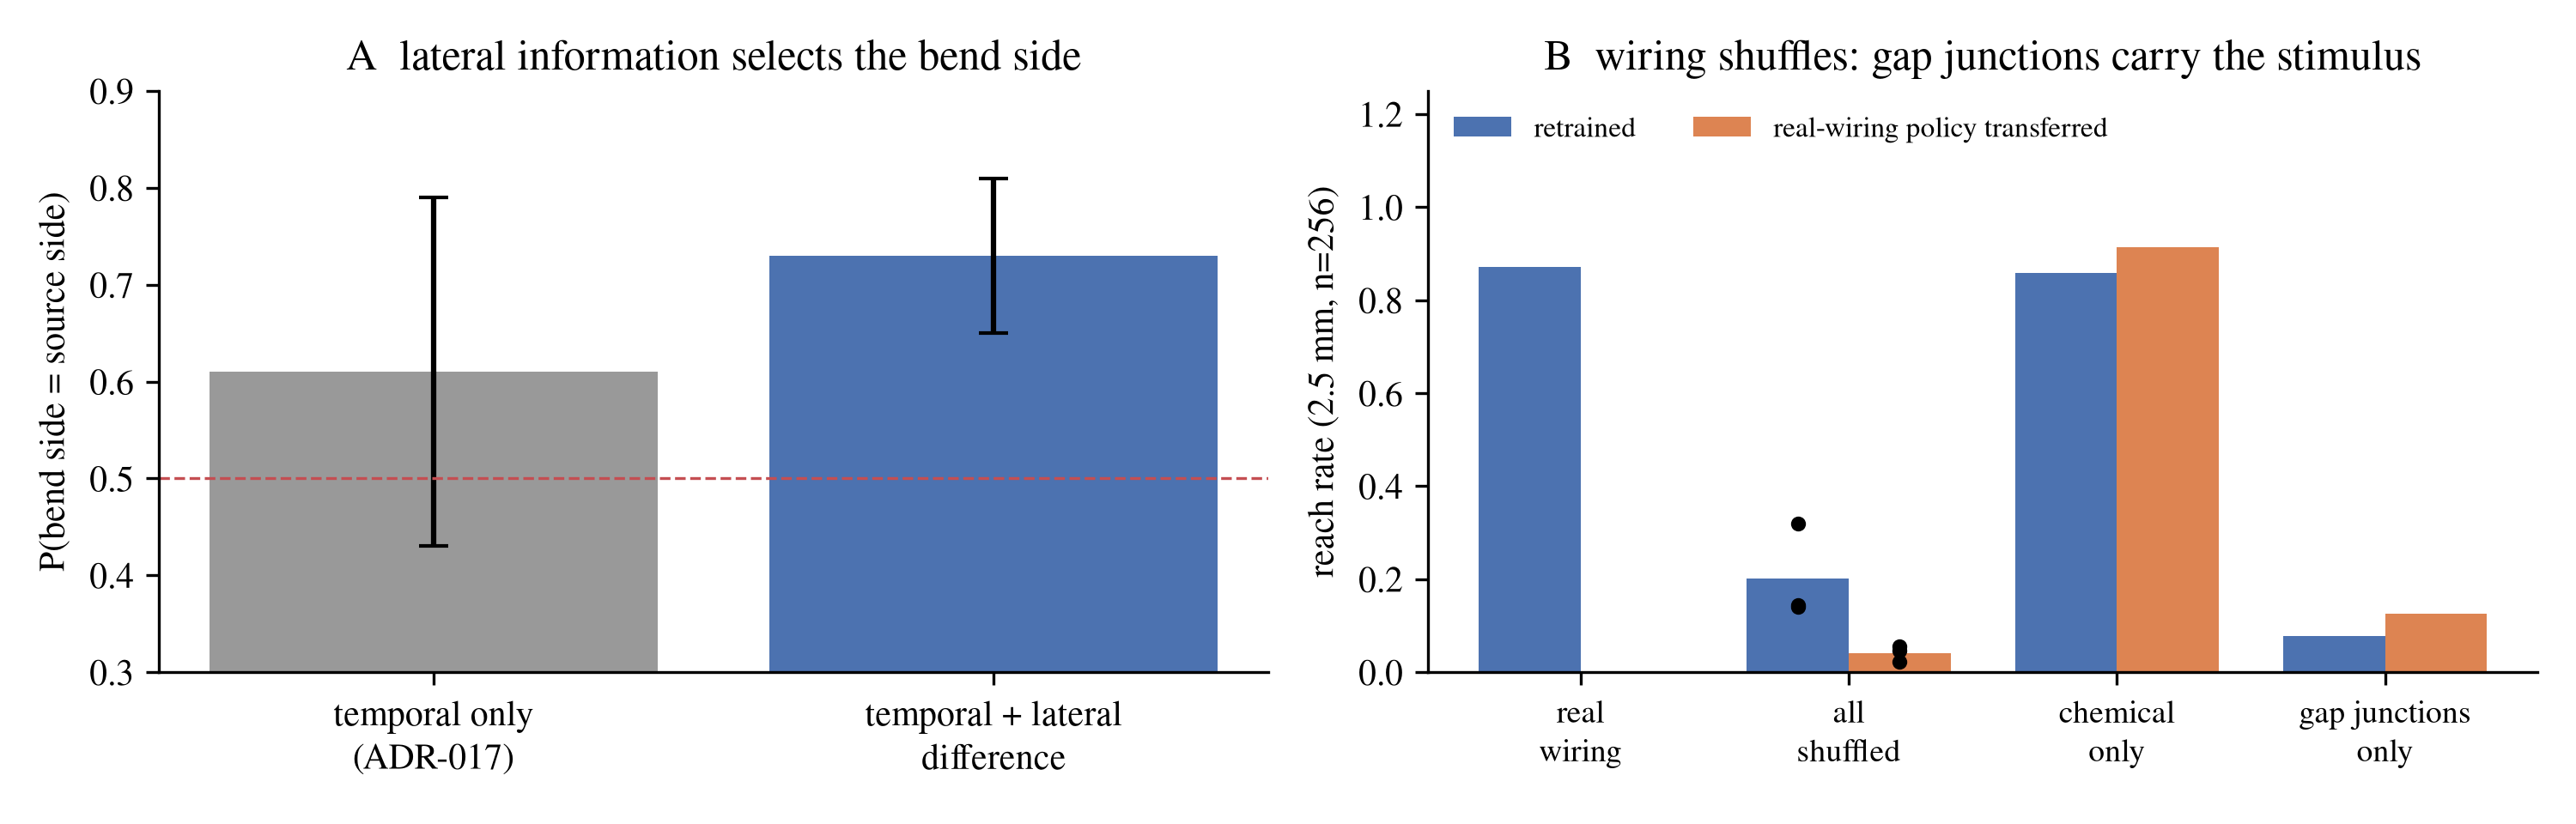
\includegraphics[width=\textwidth]{fig6_lateral_and_wiring.png}
\caption{\textbf{Lateral information and wiring controls.} (A) Per-episode probability that the deep bend is toward the source, with and without lateral information (mean $\pm$ s.d., 128 episodes). (B) Reach rates for real, fully shuffled, chemical-only shuffled and gap-junction-only shuffled wiring, retrained and with the real-wiring policy transferred.}
\label{fig6}
\end{figure}

% ---------------------------------------------------------------- References
\raggedright
\begin{thebibliography}{99}
\bibitem{r1} Izquierdo EJ, Beer RD. Connecting a connectome to behavior: an ensemble of neuroanatomical models of \textit{C. elegans} klinotaxis. PLoS Comput Biol. 2013;9(2):e1002890. doi:10.1371/journal.pcbi.1002890
\bibitem{r2} Randi F, Sharma AK, Dvali S, Leifer AM. Neural signal propagation atlas of \textit{Caenorhabditis elegans}. Nature. 2023;623(7986):406--414. doi:10.1038/s41586-023-06683-4
\bibitem{r3} Gourgou E, Adiga K, Goettemoeller A, Chen C, Hsu AL. \textit{Caenorhabditis elegans} learning in a structured maze is a multisensory behavior. iScience. 2021;24(4):102284. doi:10.1016/j.isci.2021.102284
\bibitem{r4} White JG, Southgate E, Thomson JN, Brenner S. The structure of the nervous system of the nematode \textit{Caenorhabditis elegans}. Philos Trans R Soc Lond B Biol Sci. 1986;314(1165):1--340. doi:10.1098/rstb.1986.0056
\bibitem{r5} Cook SJ, Jarrell TA, Brittin CA, Wang Y, Bloniarz AE, Yakovlev MA, et al. Whole-animal connectomes of both \textit{Caenorhabditis elegans} sexes. Nature. 2019;571(7763):63--71. doi:10.1038/s41586-019-1352-7
\bibitem{r6} Gleeson P, Lung D, Grosu R, Hasani R, Larson SD. c302: a multiscale framework for modelling the nervous system of \textit{Caenorhabditis elegans}. Philos Trans R Soc B. 2018;373(1758):20170379. doi:10.1098/rstb.2017.0379
\bibitem{r7} Boyle JH, Berri S, Cohen N. Gait modulation in \textit{C. elegans}: an integrated neuromechanical model. Front Comput Neurosci. 2012;6:10. doi:10.3389/fncom.2012.00010
\bibitem{r8} Salimans T, Ho J, Chen X, Sidor S, Sutskever I. Evolution strategies as a scalable alternative to reinforcement learning. arXiv:1703.03864 [stat.ML]. 2017.
\bibitem{r9} Pierce-Shimomura JT, Morse TM, Lockery SR. The fundamental role of pirouettes in \textit{Caenorhabditis elegans} chemotaxis. J Neurosci. 1999;19(21):9557--9569. doi:10.1523/JNEUROSCI.19-21-09557.1999
\bibitem{r10} Iino Y, Yoshida K. Parallel use of two behavioral mechanisms for chemotaxis in \textit{Caenorhabditis elegans}. J Neurosci. 2009;29(17):5370--5380. doi:10.1523/JNEUROSCI.3633-08.2009
\bibitem{r11} Kramer TS, Wan FK, Pugliese SM, Atanas AA, Hiser AW, Luo J, et al. Neural sequences underlying directed turning in \textit{Caenorhabditis elegans}. Nat Neurosci. 2026;29:1408--1424. doi:10.1038/s41593-026-02257-5
\bibitem{r12} Rozemuller WM, Werner S, Costa AC, O'Shaughnessy L, Stephens GJ, Shimizu TS. Statistics of \textit{C. elegans} turning behavior reveals optimality under biasing constraints. eLife reviewed preprint 96143. 2024. doi:10.7554/eLife.96143.1
\bibitem{r13} Gray JM, Hill JJ, Bargmann CI. A circuit for navigation in \textit{Caenorhabditis elegans}. Proc Natl Acad Sci USA. 2005;102(9):3184--3191. doi:10.1073/pnas.0409009101
\bibitem{r14} Park S, Hwang H, Nam SW, Martinez F, Austin RH, Ryu WS. Enhanced \textit{Caenorhabditis elegans} locomotion in a structured microfluidic environment. PLoS ONE. 2008;3(6):e2550. doi:10.1371/journal.pone.0002550
\bibitem{r15} Taylor SR, Santpere G, Weinreb A, Barrett A, Reilly MB, Xu C, et al. Molecular topography of an entire nervous system. Cell. 2021;184(16):4329--4347. doi:10.1016/j.cell.2021.06.023
\bibitem{r16} Fenyves BG, Szil\'agyi GS, Vassy Z, S\H{o}ti C, Csermely P. Synaptic polarity and sign-balance prediction using gene expression data in the \textit{Caenorhabditis elegans} chemical synapse neuronal connectome network. PLoS Comput Biol. 2020;16(12):e1007974. doi:10.1371/journal.pcbi.1007974
\bibitem{r17} Turek M, Besseling J, Spies JP, K\"onig S, Bringmann H. Sleep-active neuron specification and sleep induction require FLP-11 neuropeptides to systemically induce sleep. eLife. 2016;5:e12499. doi:10.7554/eLife.12499
\end{thebibliography}

\end{document}
